
%================================================================
\chapter{Simulation-Based Inference}\label{chap:sbi}
%================================================================

Computational neuroscientists have developed complex mechanistic models to describe neural phenomena of interest. Many mechanistic models are defined through simulators which describe how the process generates data. However, simulators are poorly suited for inference and lead to challenging inverse problems. Standard Bayesian inference is performed within the context of a statistical model from which the likelihood can be derived. Likelihoods are generally intractable or computationally infeasible for simulator models, which makes the typical approach to inference inaccessible. 

In this chapter we discuss \textit{simulation-based inference} (SBI), that is, algorithms that avoid explicit likelihood evaluations by instead using model simulations. SBI is perhaps best known under the moniker \textit{likelihood-free inference} (LFI). Nevertheless, we prefer the term SBI to LFI as the latter indicates that the likelihood is not present at all, which we will see is not the case.

From this chapter and onwards, there will be a minor notational tweak. In order to avoid ambiguity, observed data will be denoted by $y_\mathrm{obs}$ and simulated data, generated by the simulator model, by $y_\mathrm{sim}$.


%=============================================================== 
\section{Likelihood-Based vs. Simulation-Based}
%=============================================================== 

In this section, we detail the differences between likelihood-based and simulation-based inference. The content of this section is based on \cite{abc_handbook}, \cite{sbi_review} and \cite{snl_thesis}.


Suppose a data-generating process is controlled by parameters $\theta$, and the process generates data $y$ when run forward. We assume that the process defines the conditional likelihood function $\lhood$ for every setting of $\theta$. Given an observation $y_\mathrm{obs}$, the problem of interest is to infer parameter settings compatible with $y_\mathrm{obs}$. That is, we want to compute the posterior density $\pi \qty(\theta \mid y_\mathrm{obs})$  obtained by Bayes' theorem (\autoref{eq:bayes_unnorm}). The choice of inference algorithm primarily depends on how the data-generating process is modelled. 

A purely statistical model, or an \textit{explicit model}, describes the likelihood $p \qty(y_\mathrm{obs} \mid \theta)$ of the process given values for $y_\mathrm{obs}$ and $\theta$. With an explicit model, the posterior $\pi \qty(\theta \mid y_\mathrm{obs})$ is, in general, easily evaluated using Bayes' theorem. Samples from the posterior can be generated using Bayesian computation methods such as Markov chain Monte Carlo algorithms, as discussed in \cref{sec:bayesian_computation}. Such methods are referred to as \textit{likelihood-based inference} methods, as they explicitly evaluate the likelihood.   

On the other hand, a \textit{simulator model}, or an \textit{implicit model}, describes how the process generates data. Many mechanistic models are defined through simulator models. For any parameter setting $\theta$, a simulator model can be run forward to generate samples from the likelihood $p \qty(y_\mathrm{obs} \mid \theta)$. Unlike for explicit models, implicit simulator models generally have intractable or computationally infeasible likelihoods. The complexity or absence of the associated likelihood typically arises from it involving computationally expensive or intractable integrals, or that the simulator's internal states are unavailable. In order to perform inference on a simulator model, methods using simulations from the model rather than likelihood evaluations are needed. Such methods are referred to as \textit{simulation-based inference} methods.

In general, simulation-based methods are less efficient than likelihood-based as the former can require lots of simulations to produce accurate results. One of the main topics of research in simulation-based inference is how to reduce the required number of simulations without sacrificing inference quality.


%================================================================
\section{Approximate Bayesian Computation}\label{sec:abc}
%================================================================ 

%Approximate Bayesian Computation (ABC) constitutes a class of computational algorithms rooted in Bayesian statistics that can be used to evaluate posterior distributions of model parameters without having to explicitly calculate likelihoods. ABC algorithms approximate the likelihood by assessing how likely it is the model could have produced the observed data. This is done by comparing simulated data, generated by the simulator, to the observed data. The simulations that do not reproduce the observed data within a distance specified by a tolerance are discarded. 

Approximate Bayesian Computation (ABC) constitutes a class of computational algorithms rooted in Bayesian statistics that can be used to evaluate posterior distributions of model parameters without having to explicitly calculate likelihoods. In this section we discuss ABC and its two fundamental algorithms: the original \textit{rejection ABC} algorithm and the more sophisticated \textit{Markov chain Monte Carlo (MCMC) ABC} algorithm. 

The content of this section is mainly based on material from \cite{abc_handbook}.

%=============================================================== 
\subsection{The ABC of Approximate Bayesian Computation}
%=============================================================== 

Given observed data $\yobs$, a simulator model $\mathrm{M}(\theta)$ with parameters $\theta$ having prior $\pi(\theta)$, we seek an algorithm to sample from the posterior $\pi \qty(\theta \mid \yobs) \propto p \qty(\yobs \mid \theta) \pi(\theta)$. This can be achieved by using the \textit{rejection sampling algorithm}: 

\begin{algorithm}[H]
\caption{Rejection sampler}
\label{alg:rej_sampler1}
\SetAlgoLined
\DontPrintSemicolon
 % Algorithm 
 \nl Sample $\theta \sim \pi (\theta)$.\;
 \nl Accept $\theta$ with probability proportional to the likelihood $p\qty(\yobs \mid \theta)$.\;
\end{algorithm}

\cref{alg:rej_sampler1} can be made more general and avoid the need to explicitly compute probabilities by using the following, stochastically equivalent, formulation: 

\begin{algorithm}[H]
\caption{General rejection sampler}
\label{alg:rej_sampler2}
\SetAlgoLined
\DontPrintSemicolon
 % Algorithm 
\nl Sample $\theta \sim \pi (\theta)$.\;
\nl Simulate data $\ysim$ from $\mathrm{M}(\theta)$.\;
\nl Accept $\theta$ if $\ysim = \yobs$.\;
\end{algorithm}

\cref{alg:rej_sampler2} is due to Rubin \cite{Rubin}. The chance of the outcome $\ysim = \yobs$ will, however, be vanishingly small for most problems, and thus vastly time consuming to compute. \cref{alg:rej_sampler2} will therefore, typically, not be an efficient algorithm. This is where the approximation to Bayesian computation comes into play. We define a discrepancy metric $\rho(\cdot, \cdot)$ to compare the simulated and observed data and a tolerance $\epsilon \geq 0$. The approximate Bayesian computation (ABC) algorithm is then: 

\begin{algorithm}[H]
\caption{Approximate rejection sampler}
\label{alg:rej_sampler3}
\SetAlgoLined
\DontPrintSemicolon
 % Algorithm 
 \nl Sample $\theta \sim \pi (\theta)$. \;
 \nl Simulate data $\ysim$ from $\mathrm{M}(\theta)$. \;
 \nl Compute $\rho \equiv \rho \qty(\ysim, \yobs)$, and accept $\theta$ as an approximate draw from $\pi \qty(\theta \mid \yobs)$ if $\rho \leq \epsilon$. \;
\end{algorithm}

\cref{alg:rej_sampler3} is called the \textit{rejection ABC algorithm} and was first proposed by Tavaré et al. in \cite{Tavare} and developed by Pritchard et al. in \cite{Pritchard}. In the scheme of Pritchard et al., the simulated and observed data were compared through a choice of summary statistics. We will discuss the algorithm in more detail in the next section. 


%=============================================================== 
\subsection{Rejection ABC}
%=============================================================== 

\textit{Rejection ABC}, as outlined in \cref{alg:rej_sampler3}, is a rejection sampling algorithm for obtaining independent samples from the approximate posterior $ \pi_\mathrm{ABC} \qty(\theta \mid \rho \qty(\ysim, \yobs) \leq \epsilon)$, where $\rho \qty(\cdot, \cdot)$ is a discrepancy metric, e.g. the Euclidean distance, and $\epsilon \geq 0$ a tolerance. The algorithm proceeds by first sampling a set of parameters $\theta$ from the prior, then generate simulated data $\ysim$ under the simulator model $\mathrm{M}\qty(\theta)$ specified by the sampled $\theta$, and finally accepting and retaining $\theta$ if the distance between $\ysim$ and $\yobs$ is no more than $\epsilon$. If $\rho \qty(\ysim, \yobs) = 0$, then $\ysim = \yobs$, and the accepted $\theta$ is a sample from the true posterior. The tolerance parameter $\epsilon$ thus controls the trade-off between estimation accuracy and computational efficiency. With sufficiently small $\epsilon$, the accepted samples follow the exact posterior more closely, though the algorithm accepts less often. On the other hand, the algorithm accepts more often with a large $\epsilon$, but the accepted samples might yield a replica of the prior.  

Stochastically matching $\ysim$ and $\yobs$ becomes increasingly difficult with increasing dimensionality of the data. In order to operate efficiently, ABC algorithms require a compression of the data into low-dimensional summary statistics $s = S(y)$. A summary statistic that contains the same amount of information about model parameters as the whole dataset, is referred to as being a sufficient statistic $\tilde{s}$. Thus, 

\begin{equation}
\begin{aligned}
    \pi \qty(\theta | \yobs ) &= \lim_{\epsilon \to 0} \pi_\mathrm{ABC} \qty(\theta \mid \rho \qty (\ysim, \yobs) \leq \epsilon) 
    \\
    &= \lim_{\epsilon \to 0} \pi_\mathrm{ABC} \qty(\theta \mid \rho \qty (\tilde{s}_\mathrm{sim}, \tilde{s}_\mathrm{obs}) \leq \epsilon)
    \\
    &\approx \lim_{\epsilon \to 0} \pi_\mathrm{ABC} \qty(\theta \mid \rho \qty (s_\mathrm{sim}, s_\mathrm{obs}) \leq \epsilon)
\end{aligned}
\end{equation}

The choice of summary statistics is crucial for the performance of ABC algorithms, and the optimal choice is a minimal sufficient summary statistic. It is common to use the Fisher-Neyman factorization theorem to determine whether or not a summary statistic is sufficient. The theorem is based on being able to re-express the likelihood as a function of the sufficient summary statistic and data. Unfortunately, in the context of simulation-based inference, the likelihood is unavailable and we cannot examine a summary statistic to determine if the Fisher-Neyman factorization theorem holds. However, if powerful low-dimensional summary statistics are established, ABC algorithms can still offer a reasonable performance. The dimension of the vector of summary statistics $s$ should be large enough so that it capture as many important features of the observed data as possible, but also low enough so the curse of dimensionality of matching $\ssim$ and $\sobs$ is avoided. 

\autoref{fig:abc_illustration} gives a conceptual overview of the rejection ABC algorithm in a two-dimensional summary statistic space. Having observed data $\yobs$ provided by nature and reduced it to a summary statistic $\sobs$ (the blue dot), we sample parameter values $\theta \sim \prior$, generate simulated data $\ysim$ through the simulator $\mathrm{M}(\theta)$, compute the simulated summary statistic $\ssim$ and compare with the observation. Here, the discrepancy metric is the Euclidean distance, and the acceptance region amounts to a circle (indicated by the shaded grey circle) with center according to the observation and radius determined by the tolerance $\epsilon$. The $\theta$ that correspond to $\ssim$ within this circle are accepted (the green dots), and those outside the circle are rejected (the red dots). 

\begin{figure}[!htb]
    \centering 
    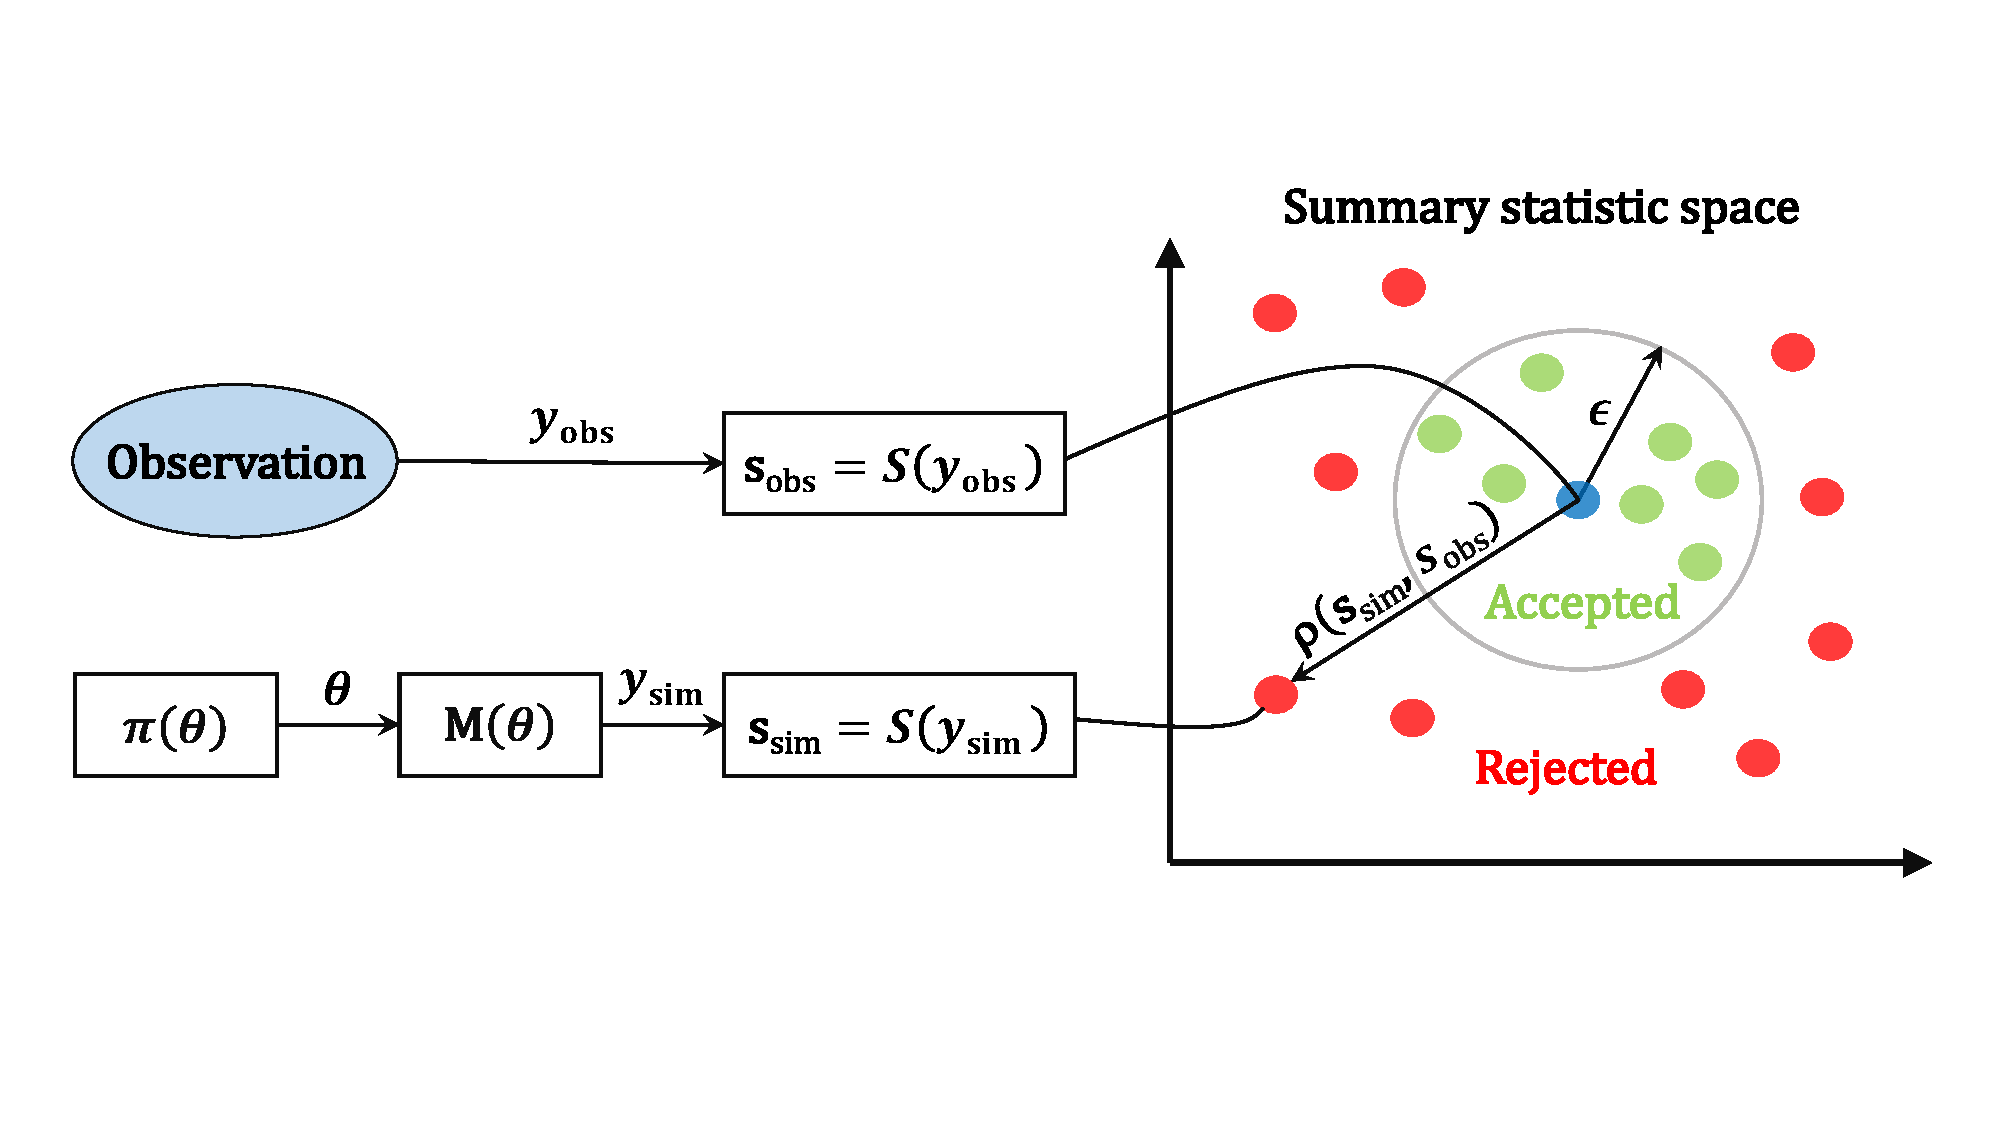
\includegraphics[scale=0.4]{ABC_illustration}
    \caption{A conceptual overview of rejection ABC in 2D summary statistic space. The discrepancy metric is the Euclidean distance, which has a circular acceptance region with the observed summary statistic $\sobs$ as center (blue dot) and tolerance $\epsilon$ as radius. The parameters $\theta$ with corresponding simulated summary statistics $\ssim$ that fall within the acceptance region are accepted (green dots), and those outside are rejected (red dots). See text for additional details.}
    \label{fig:abc_illustration}
    \source{Adapted from Fig. 3 in \cite{abc_figure}.}
\end{figure}

\cref{alg:rej_abc} summarizes the full rejection ABC algorithm.

\begin{algorithm}[H]
\caption{Rejection ABC}
\label{alg:rej_abc}
\SetAlgoLined
\DontPrintSemicolon
 % Algorithm 
 \textbf{Inputs\,:}\;
 \vspace{-5mm}
 \begin{itemize}
     \item An observation $\yobs$. 
     \item A simulator model $\mathrm{M}(\theta)$ with parameters $\theta$ having prior $\prior$.
     \item A discrepancy metric $\rho(\cdot, \cdot)$ and threshold $\epsilon \geq 0$. 
     \item A summary statistics function $S(y)$. 
     \item An integer $N>0$.
 \end{itemize}
 
 \vspace{5mm}
 \textbf{Sampling\,:}\;
 \For{$i=1, ..., N$}{ 
 \nl Sample $\theta \sim \prior$. \; 
 \nl Simulate data $\ysim $ from $M(\theta)$. \;
 \nl Calculate $\rho \equiv \rho \qty(S \qty(\ysim), S \qty(\yobs)) = \rho \qty(\ssim, \sobs)$. \; 
 \vspace{2mm}
 \eIf{$\rho \leq \epsilon$}{
   \nl Accept $\theta$. \;
   }{
   \nl Go to 1. \;
  }
 }
\end{algorithm}


%=============================================================== 
\subsection{Markov Chain Monte Carlo ABC}
%=============================================================== 

In Rejection ABC, the proposal parameters are sampled from the prior. Although sampling from the prior is efficient, the efficiency of the overall procedure will be determined by whether the prior is chosen so that it is of a similar shape and location as the desired posterior. The acceptance rate will be low if the approximate posterior is significantly narrower than the prior, as is often the case. The rejection ABC algorithm will thus become more computationally inefficient as more of the expensive data generation becomes necessary. In this case, we might choose to develop a recursive strategy where the quality of previous candidates in our sampling algorithm can be used to guide the candidate generation process. Basing proposal samples off of previous states is precisely the strategy behind conventional Markov chain Monte Carlo (MCMC) methods, as we introduced in \cref{sec:bayesian_computation}. 

Beaumont et al. \cite{Beaumont} were the first to both extend the ABC approach to use MCMC methods and use the term \textit{Approximate Bayesian Computation}. \cref{alg:mcmcabc} summarizes the \textit{MCMC ABC} algorithm with Metropolis sampling (also discussed in \cref{sec:bayesian_computation}). To perform Metropolis sampling in the simulation-based context, we calculate the probability of accepting the proposal $\theta^*$ by evaluating: 

\begin{equation}\label{eq:abc_metropolis}
    \alpha = \begin{cases}
    \min \qty(1, \frac{\pi \qty(\theta^*)}{\pi \qty(\theta_{t-1})}) \qquad &\text{if } \rho \qty(\ssim, \sobs) \leq \epsilon 
    \\
    0 \qquad &\text{if } \rho \qty(\ssim, \sobs) > \epsilon 
    \end{cases}
\end{equation}

Similarly to rejection ABC, the acceptance probability of MCMC ABC decreases as $\epsilon$ becomes small. Moreover, the performance of MCMC ABC strongly depends on the selection of proposal and prior density. 

\begin{algorithm}[!htb]
\caption{Markov chain Monte Carlo ABC with Metropolis sampler}
\label{alg:mcmcabc}
\SetAlgoLined
\DontPrintSemicolon
 % Algorithm 
 \textbf{Inputs\,:}\;
 \vspace{-5mm}
 \begin{itemize}
    \item An observation $\yobs$. 
     \item A simulator model $\mathrm{M}(\theta)$ with parameters $\theta$ having prior $\prior$.
     \item A symmetric Markov proposal density $q \qty(\theta^* \mid \theta)$.
     \item A discrepancy metric $\rho(\cdot, \cdot)$ and threshold $\epsilon \geq 0$. 
     \item A summary statistics function $S(y)$. 
     \item An integer $N>0$.
 \end{itemize}
 
 \vspace{5mm}
 \textbf{Initialize\,:}\;
 \nl Sample $\theta_0$ by performing one iteration of rejection ABC (\cref{alg:rej_abc}).\;

 \vspace{5mm}
 \textbf{Sampling\,:}\;
 \For{$t=1, ..., N$}{ 
 \nl Generate proposal $\theta^* \sim q \qty(\theta^* \mid \theta_{t-1})$. \; 
 \nl Simulate data $\ysim $ from $M \qty(\theta^*)$. \;
 \nl Calculate $\rho \equiv \rho \qty(S \qty(\ysim), S \qty(\yobs)) = \rho \qty(\ssim, \sobs)$. \; 
 \nl Calculate acceptance criterion $\alpha$ (\autoref{eq:abc_metropolis}). \;
 \nl Sample $u \sim \mathrm{U}(0,1)$. \; 
 \vspace{2mm}
 \eIf{$u \leq \alpha$ and $\alpha \neq 0$}{
 \nl  $\theta_t = \theta^*$\;
   }{
  \nl $\theta_t = \theta_{t-1}$\;
  }
 }
\end{algorithm}

%=============================================================== 
\section{Regression Adjustment}
%=============================================================== 

In this section, we discuss a post-sampling refinement called \textit{regression adjustment}, first proposed by Beaumont et al. in \cite{Beaumont}. The goal of the method is to improve the posterior approximation. Usually, we choose summary statistics with a systematic relationship to the model parameters. The idea behind regression adjustment is to correct the accepted posterior samples based on this relationship and the distance between the simulated and observed summary statistics. The content of this section is based on material from \cite{Beaumont}, \cite{abc_handbook} and \cite{lfi_cogsci}. 

%=============================================================== 
\subsection{Linear Regression Adjustment}
%=============================================================== 

Let $\sobs = \qty(s_{\mathrm{obs}, 1}, ..., s_{\mathrm{obs}, m})$ be the vector of observed summary statistics, where we let $s_{\mathrm{obs}, j}$ denote the $j$th summary statistic and assume appropriate scaling of the summary statistics, e.g., to equalize variances. An ABC algorithm generates a vector of parameters $\theta = \qty(\theta_1, ..., \theta_l)$ by comparing the vectors of simulated summary statistics $\ssim = \qty(s_{\mathrm{sim}, 1}, ..., s_{\mathrm{sim}, m})$ with the observation. The posterior approximation of the $k$th model parameter, $\theta_k$, is a vector consisting of $n$ accepted samples, $\theta_k = \qty(\theta_k^{(1)}, ..., \theta_k^{(n)})$. In the following, we let $\theta^{(i)}$ indicate the $i$th accepted sample of model parameters with $i=1, ..., n$. Furthermore, assume we retain the simulated summary statistics associated with the accepted $\theta^{(i)}$ sample, such that we also have the vector $\ssim^{(i)}$, $i=1, ..., n$. Thus, we have $n$ pairs of $\qty(\theta^{(i)}, \ssim^{(i)})$.

It is convenient to start our discussion of regression adjustment based on standard linear regression to explain the main ideas. The first objective is to model the relationship between the $m$-dimensional vector of summary statistics and the $l$-dimensional vector of model parameters, where each vector component itself is an $n$-dimensional vector consisting of the associated accepted samples. A model for linearly regressing the summary statistics on the obtained posterior samples is: 

\begin{equation}\label{eq:linreg_model}
    \theta^{(i)} = \alpha + \qty(\ssim^{(i)} - \sobs)^\mathrm{T} \beta + \xi^{(i)}, \qquad i=1, ..., n
\end{equation} 

where $\alpha$ is the intercept, $\beta$ the vector of regression coefficients and $\xi^{(j)}$ the residual assumed to be uncorrelated with mean zero and common variance. No other distributional assumptions are made about $\xi^{(i)}$ and hence $\theta^{(i)}$. When $\ssim^{(i)} = \sobs$, the $\theta^{(i)}$ are samples from the desired posterior with mean $\alpha$. The least squares estimate of $(\alpha, \beta)$ is:

\begin{equation}\label{eq:linreg_sol}
    \qty(\hat{\alpha}, \hat{\beta}) = \qty(X^\T X)^{-1} X^\T \theta,
\end{equation}

where $X$ is the matrix of summary statistics augmented with a column of ones: 

\begin{equation*}
    X = \begin{bmatrix}
    1 & s_{\mathrm{sim}, 1}^{(1)} - s_{\mathrm{obs}, 1} & s_{\mathrm{sim}, 2}^{(1)} - s_{\mathrm{obs}, 2} & \dots & s_{\mathrm{sim}, m}^{(1)} - s_{\mathrm{obs}, m}
    \\
    1 & s_{\mathrm{sim}, 1}^{(2)} - s_{\mathrm{obs}, 1} & s_{\mathrm{sim}, 2}^{(2)} - s_{\mathrm{obs}, 2} & \dots & s_{\mathrm{sim}, m}^{(2)} - s_{\mathrm{obs}, m}
    \\
    \vdots & \vdots & \vdots & \ddots & \vdots 
    \\
    1 & s_{\mathrm{sim}, 1}^{(n)} - s_{\mathrm{obs}, 1} & s_{\mathrm{sim}, 2}^{(n)} - s_{\mathrm{obs}, 2} & \dots & s_{\mathrm{sim}, m}^{(n)} - s_{\mathrm{obs}, m}
    \end{bmatrix}.
\end{equation*}

The strategy is then to adjust the set of posterior samples $\theta$ to have mean $\alpha$ while simultaneously correcting for the trend in the relationship between parameters and summary statistics. It follows from \autoref{eq:linreg_model} that the corrected posterior sample $\tilde{\theta}^{(i)}$ defined by 

\begin{equation}\label{eq:linreg_adj}
    \tilde{\theta}^{(i)} = \theta^{(i)} \qty(\ssim^{(i)} - \sobs)^\mathrm{T} \hat{\beta}
\end{equation}

form an approximate random sample from the posterior $\pi \qty(\theta \mid \sobs)$. If the relationship between the model parameters and the summary statistics is truly linear, which also implies that the summary statistics are sufficient, this will be exact (assuming that also the distributional assumptions about $\xi^{(i)}$ are met and the sample size is large so that $\qty(\hat{\alpha}, \hat{\beta})=(\alpha, \beta)$). It should be noted that $\hat{\alpha}$ can be interpreted as a point estimate of $\theta$ since it is an estimate of the posterior mean.

It may not be immediately evident how this correction helps to improve the posterior approximation, so here comes an explanation: A crucial limitation of the ABC algorithms is that they can only handle a small number of summary statistics. However, in order to constrain the model parameters accurately we might need several informative summary statistics. As a consequence, we usually have a trade-off between prohibitively low acceptance rates or large tolerances which can distort the approximation. This arises from the fact that $\ssim$ are treated equally whenever $\rho \qty(\ssim, \sobs) \leq \epsilon$, regardless of the proximity between $\ssim$ and $\sobs$. The idea of regression adjustment is to learn a regression model and then correct the accepted simulations as if they were sampled from $\pi_\mathrm{ABC} \qty(\theta \mid \rho \qty(\ssim, \sobs) \leq \epsilon)$ with $\epsilon=0$. With this insensitivity to $\epsilon$, we can also increase the number of summary statistics and thus potentially extract more information from the data. \autoref{fig:reg_adj_figure} illustrates linear regression adjustment of a univariate parameter $\theta$.


\begin{figure}[!htb]
    \centering
    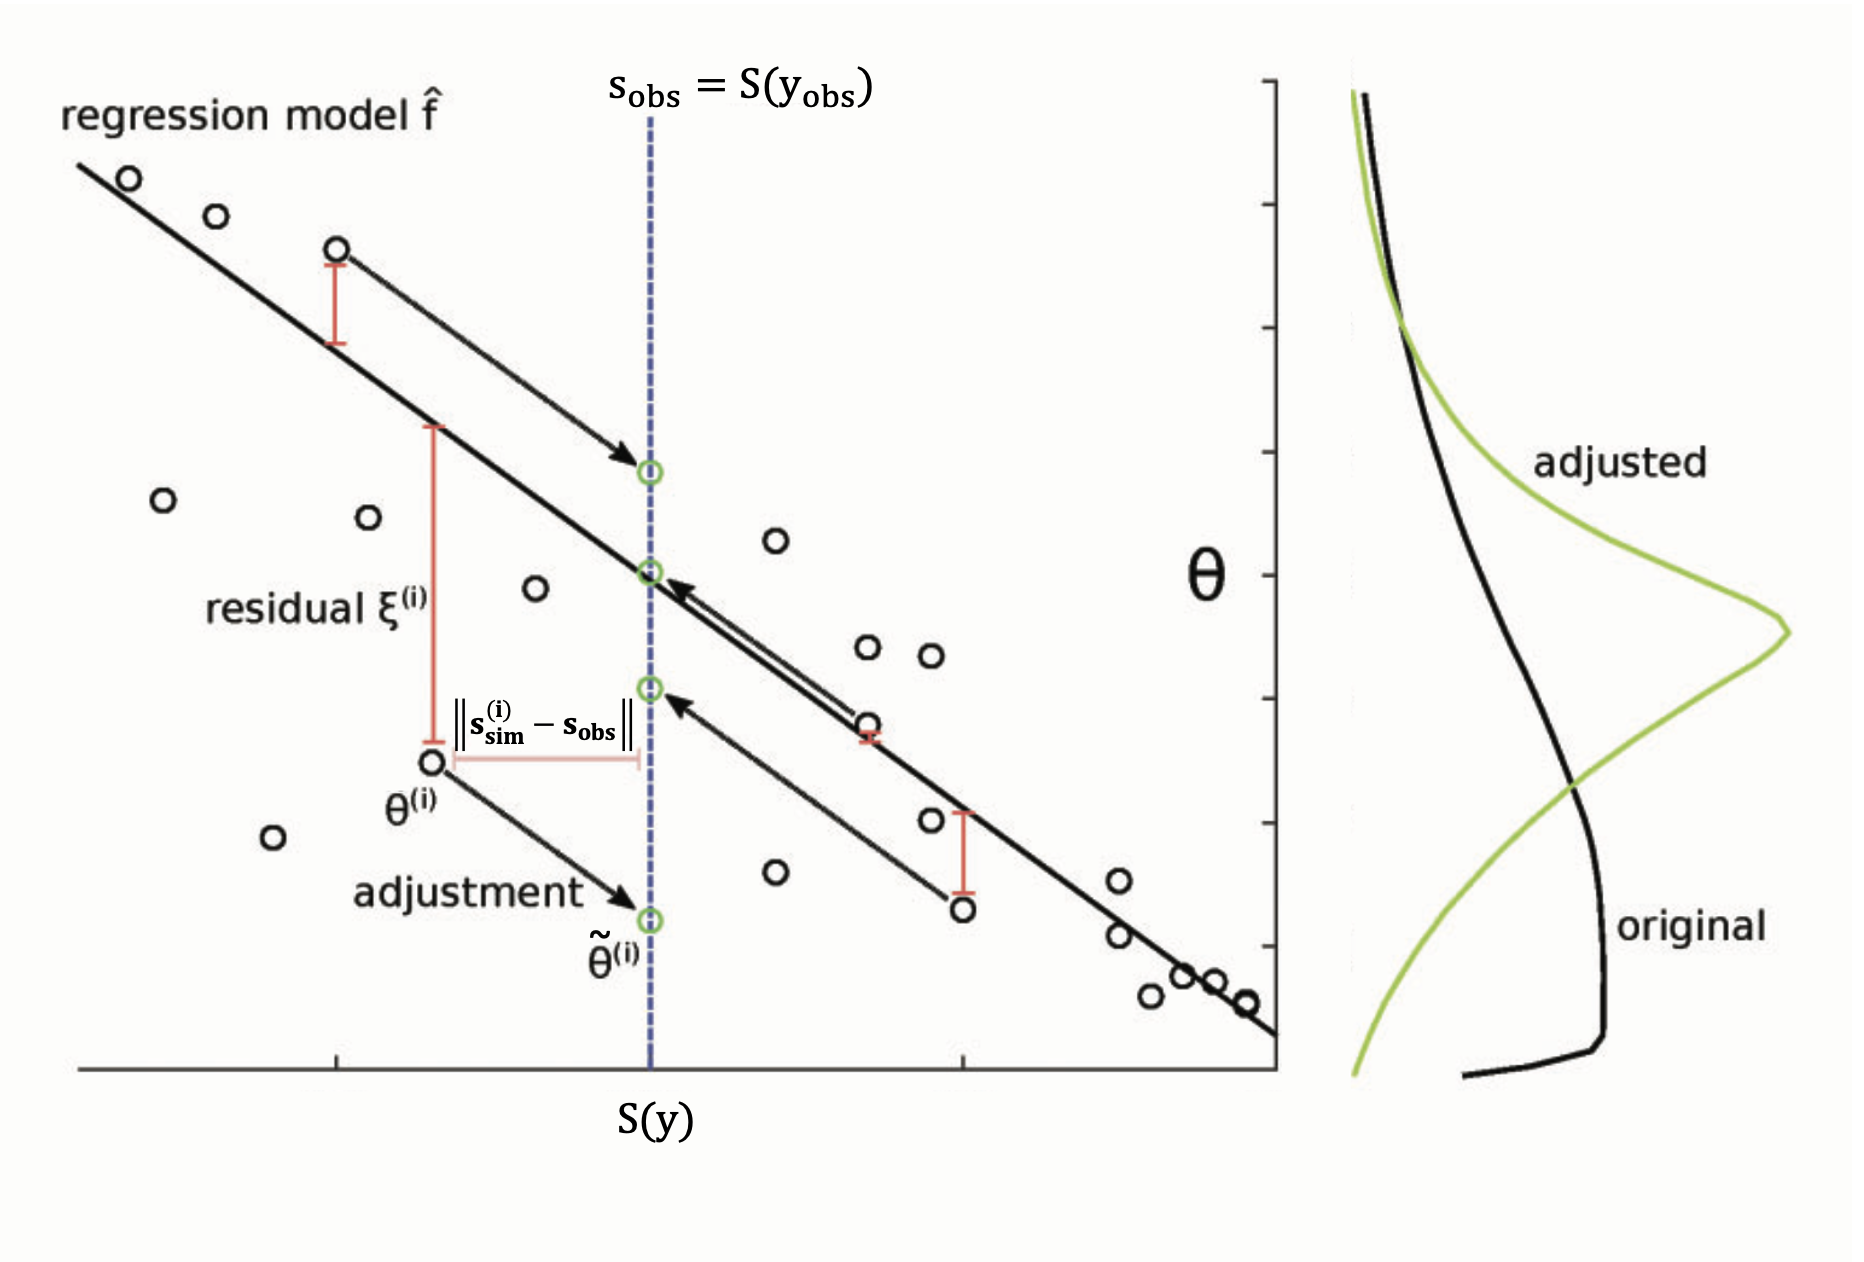
\includegraphics[scale=0.4]{regression_adj}
    \caption{Illustration of linear regression adjustment of a univariate parameter $\theta$. The vertical blue dashed line indicates the observed summary statistic, $\sobs$. First, a regression model $\hat{f}$ is learned and then, based on $\hat{f}$, all accepted posterior samples $\theta^{(i)}$ are corrected as if they were sampled from $\pi_\mathrm{ABC} \qty(\theta \mid \rho \qty(\ssim, \sobs) \leq \epsilon)$ with $\epsilon=0$. Note that the residuals $\xi^{(i)}$ are preserved. Corrected samples are denoted by $\tilde{\theta}^{(i)}$, and the shift in values are indicated by the black arrows pointing to the positions of the corrected values (green circles). The original posterior density is shown on the right (black curve) together with the adjusted posterior (green curve). 
    }
    \label{fig:reg_adj_figure}
    \source{Modified from Fig. 9 in \cite{reg_adj_figure}.}
\end{figure}



%=============================================================== 
\subsection{Local Linear Regression Adjustment}
%=============================================================== 

Linear regression adjustment works well if the relationship between the parameters and the summary statistics is approximately linear, however this is rarely true in practice. Although, approximate linearity may be true in a localized region around $\sobs$. Thus, we can perform \textit{local linear regression}, which applies kernel smoothed (see \cref{sec:kde}) weights to each $\theta^{(i)}$ based on the distance between $\ssim^{(i)}$ and $\sobs$. That is, we localize the regression problem by defining a kernel $K\qty(\norm{\ssim^{(i)} - \sobs}/ \epsilon)$, where $\norm{\cdot}$ is the Euclidean distance and the tolerance $\epsilon$ is the bandwidth of the kernel. This guarantees that $\theta^{(i)}$ associated with $\ssim^{(i)}$ close to $\sobs$ are weighted more heavily. The kernel can assume many forms, such as the Gaussian kernel:

\begin{equation}\label{eq:gaussian_kernel_lra}
    K \qty( \frac{\norm{\ssim - \sobs}}{\epsilon} ) = \exp(-\frac{1}{2} \qty(\frac{\norm{\ssim - \sobs}}{\epsilon})^2 ),
\end{equation}

and the Epanechnikov kernel:

\begin{equation}\label{eq:epkov_kernel_lra}
    K \qty( \frac{\norm{\ssim - \sobs}}{\epsilon} )  = \begin{cases} 
    1 - \qty(\frac{\norm{\ssim - \sobs}}{\epsilon})^2 \qquad &\text{if } \norm{\ssim - \sobs} \leq \epsilon
    \\
    0 \qquad &\text{otherwise}
    \end{cases}.
\end{equation}

The weighted least squares estimate for $(\alpha, \beta)$ is: 

\begin{equation}\label{eq:locreg_sol}
    \qty(\hat{\alpha}, \hat{\beta}) = \qty(X^\T W X)^{-1} X^\T W \theta,
\end{equation}

where $W$ is the $n\times n$ weight matrix whose $i$th diagonal element is $K\qty(\norm{\ssim^{(i)} - \sobs}/ \epsilon)$ while all other elements are zero: 

\begin{equation*}
    W = \begin{bmatrix}
    K\qty(\frac{\norm{\ssim^{(1)} - \sobs}}{\epsilon}) & 0 & \dots & 0 
    \\
    0 & K\qty(\frac{\norm{\ssim^{(2)} - \sobs}}{\epsilon}) & \dots & 0 
    \\
    \vdots & \vdots & \ddots & \vdots 
    \\
    0 & 0 & \dots & K\qty(\frac{\norm{\ssim^{(n)} - \sobs}}{\epsilon})
    \end{bmatrix}
\end{equation*}

The correction is then done according to \autoref{eq:linreg_adj}, but with the weighted estimate for $\beta$ (\autoref{eq:locreg_sol}).




%===============================================================
\section{Neural Density Estimation}
%===============================================================

We reviewed some standard methods for \textit{nonparametric} density estimation in \cref{sec:densest}. Here, we introduce \textit{neural density estimation} (NDE), a \textit{parametric} density estimation method where the density estimator is an \textit{artificial neural network} (ANN). Since the posterior is a conditional density, we are in particular interested in \textit{conditional neural density estimators}. One class of conditional NDEs is \textit{normalizing flows} (NF), which is a transformation of a simple base distribution, e.g., the normal distribution, into a more complex distribution by a sequence of invertible transformations that are differentiable. NFs were popularized for density estimation by Dinh et al. in \cite{dinh2015nice}. Another general framework for modelling arbitrary conditional densities is mixture density networks (MDNs), see e.g. Bishop \cite{Bishop}, which combines a conventional feedforward ANN with a mixture density model of the target (the posterior in our case). 


%===============================================================
\subsection{Sequential Neural Posterior Estimation}
%===============================================================

Sequential Neural Posterior Estimation (SNPE) is a novel algorithm for simulation-based inference based on NDE. Dissecting all of the intricacies of SNPE, and NDE in general, is beyond the scope of this thesis. We will in this section provide an overview of the algorithm(s). For full details, we refer the reader to the original articles \cite{SNL_first}, \cite{SNPE_first} and \cite{SNPE_apt}.

SNPE targets directly learning the posterior $\posterior$ by training a conditional NDE on adaptively proposed simulations of the simulator model. Using adaptive proposals means that the parameters are not drawn from the prior $\prior$, but rather a proposal distribution $\tilde{\pi}(\theta)$ that is updated over a number of training rounds. In each round, the proposal is taken to be the approximate posterior distribution itself from the previous round. The idea behind this approach is to increase sample efficiency, as sampling parameters from the prior can lead to wasteful simulations. The use of a proposal $\tilde{\pi}(\theta)$ different from the prior $\prior$ does, however, require a correction step, as samples drawn from $\tilde{\pi}(\theta)$ no longer yield the target posterior $\posterior$ but rather the \textit{proposal posterior}:

\begin{equation}\label{eq:proposal_posterior}
    \tilde{\pi} \qty(\theta \mid y) = \posterior \frac{\tilde{\pi}(\theta) p(y)}{\prior \tilde{p}(y)},
\end{equation}

where $\tilde{p}(y) = \int \lhood \tilde{\pi}(\theta)\dd{\theta}$. Note that for $\tilde{\pi}(\theta) = \prior$, it directly follows that $\tilde{\pi} \qty(\theta \mid y) = \posterior$. 

There have been developed three main approaches to the correction step so far, leading to three versions of SNPE; SNPE-A by Papamakarios and Murray \cite{SNL_first}, SNPE-B by Lueckmann et al. \cite{SNPE_first} and SNPE-C by Greenberg et al. \cite{SNPE_apt}. All algorithms have in common that they train a neural network $F(y, \phi)$, i.e., a network with weights $\phi$ that takes as input data $y$, to learn the parameters of a family of densities $q_\psi$, where $\psi$ are distribution parameters, to estimate the posterior. They differ in what is targeted by $q_\psi$ and which loss is used for $F$. With this notation, $q_{F(y, \phi)} (\theta)$ represents an estimate of $\posterior$, and $\tilde{q}_{F(y, \phi)} (\theta)$ an estimate of $\tilde{\pi} \qty(\theta \mid y)$.

SNPE-A trains F, which is required to be a Gaussian MDN in this algorithm, to target the proposal posterior $\tilde{\pi} \qty(\theta \mid y)$ by minimizing the log likelihood loss $\mathcal{L} = - \sum_n \log q_\psi \qty(\theta_n \mid y_n)$. The learned proposal posterior $\tilde{q}_{F(y, \phi)} \qty(\theta)$ is then corrected analytically by dividing it by $\tilde{\pi}(\theta)$ and multiplying it by $\prior$. The analytical post-hoc step restricts $\tilde{\pi}(\theta)$ to be Gaussian and $\prior$ to be either Gaussian or uniform. 

SNPE-B also trains a MDN and deals with the correction step by adjusting the parameters $\theta_n$ by assigning them weights $w_n = \pi \qty(\theta_n) / \tilde{\pi}\qty(\theta_n)$. During training SNPE-B minimizes the importance weighted loss $\mathcal{L} = - \sum_n w_n \log q_\psi \qty(\theta_n \mid y_n)$, which allows for direct recovery of $\posterior$. Since there is no need for post-hoc correction, SNPE-B lifts the restrictions on $\prior$, $\tilde{\pi}(\theta)$ and $q_\psi$ placed by SNPE-A. However, the weights can have high variance, which can lead to slow or inaccurate inference due to high-variance gradients and instability during training. 

SNPE-C circumvents the issues of SNPE-A and SNPE-B by reparameterizing \autoref{eq:proposal_posterior} such that it is possible to automatically transform between estimates of $\posterior$ and $\tilde{\pi} \qty(\theta \mid y)$. Since $\tilde{\pi}(\theta \mid y) \propto \posterior \tilde{\pi}(\theta)/\prior$, SNPE-C defines:

\begin{equation}\label{eq:apt}
    \tilde{q}_{y, \phi} (\theta) = q_{F(y, \phi)} (\theta) \frac{\tilde{\pi}(\theta)}{\prior} \frac{1}{Z(y, \phi)},
\end{equation}

where $Z(y, \phi) = \int q_{F(y, \phi)} (\theta) \frac{\tilde{\pi}(\theta)}{\prior} \dd{\theta}$ is a normalization constant. The network is trained by minimizing the loss $\mathcal{L} = - \sum_n \log \tilde{q}_{y, \phi} \qty(\theta_n)$, such that both the target and proposal posteriors are recovered. SNPE-C supports a wide range of proposals and conditional NDEs, including MDNs and NFs. Its only requirement is a closed form solution of \autoref{eq:apt} for $\tilde{q}_{F(y, \phi)}$, to be optimized during training and sampled from afterwards.  

SNPE will in the following refer to the SNPE-C variant. \autoref{fig:snpe} gives a conceptual overview of the SNPE algorithm. Perhaps the two most notable features of SNPE is that it uses \textit{all} model simulations to train the network and, once trained, it can be used to predict posteriors over model parameters on any empirical data with just one forward pass through the network.

\begin{figure}[!htb]
    \centering
    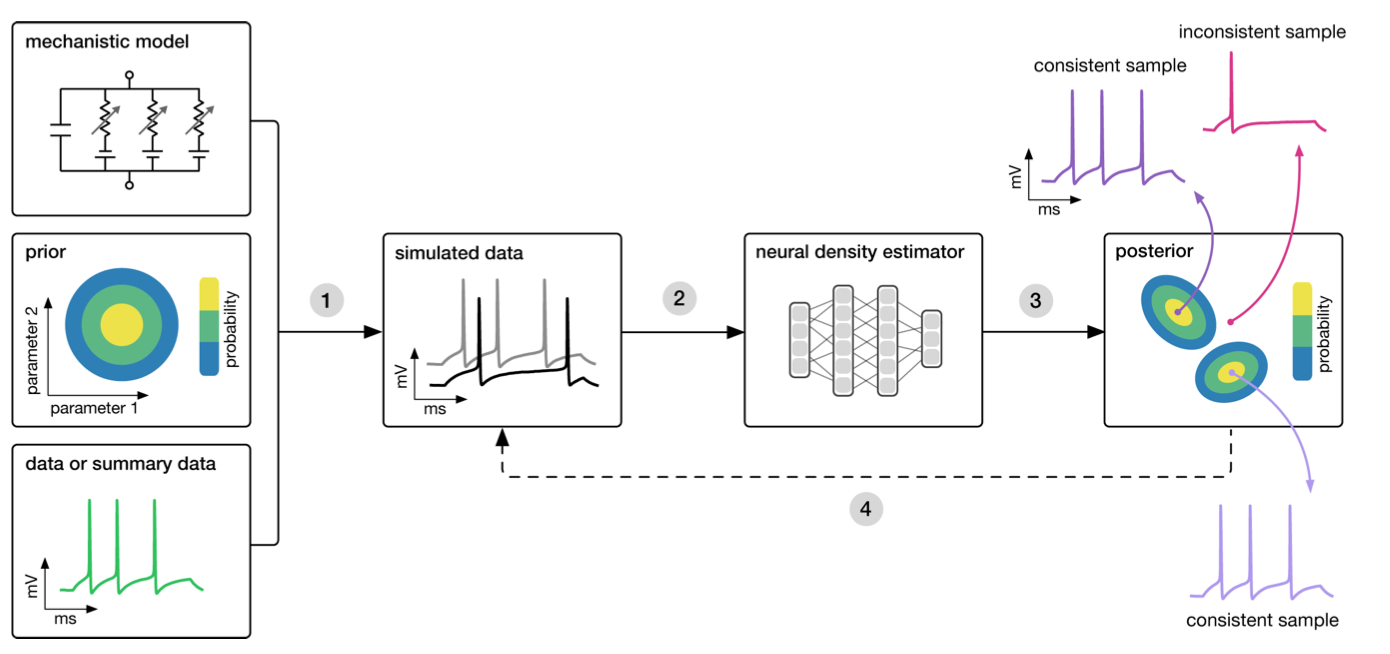
\includegraphics[scale=0.6]{snpe}
    \caption{A conceptual overview of posterior estimation via the Sequential Neural Posterior Estimation (SNPE) algorithm. SNPE takes three inputs: a simulator of the mechanistic model, priors over model parameters and observed data, either as summary statistics of or the raw data itself. The algorithm then proceeds by: (1) Sample parameters from (i) the priors in the first rounds, and (ii) the proposal distribution in subsequent rounds, and feed them to the simulator to generate simulated data; (2) Train a conditional neural density estimator (a neural network) to learn the probabilistic association between data (or summary statistics of the data) and the underlying parameters; (3) Use the density estimation network to predict the posterior distributions over model parameters consistent with the observed data; (4) Under training, the approximate posterior on simulated data is used to adaptively update the proposal distribution so that more informative simulations become likely.
    }
    \label{fig:snpe}
    \source{\cite{SNPE_applied}.}
\end{figure}














    


